% =====================================================================
%  Reporte técnico: MongoDB vs PostgreSQL JSONB bajo contención cgroups v2
%  Compilar con:  latexmk -pdf reporte_benchmark.tex   (o pdflatex x2)
%  Todas las cifras provienen de results/mediciones.csv, results/anexo_variantes.csv
%  y results/raw/<run_id>/meta.json (180 corridas reales).
% =====================================================================
\documentclass[11pt,a4paper]{article}

\usepackage[utf8]{inputenc}
\usepackage[T1]{fontenc}
\usepackage{lmodern}
\IfFileExists{spanish.ldf}{%
  \usepackage[spanish,es-noshorthands,es-tabla,es-nodecimaldot]{babel}%
}{%
  \usepackage[english]{babel}%
  \addto\captionsenglish{%
    \renewcommand{\contentsname}{Índice general}%
    \renewcommand{\listfigurename}{Índice de figuras}%
    \renewcommand{\listtablename}{Índice de tablas}%
    \renewcommand{\figurename}{Figura}%
    \renewcommand{\tablename}{Tabla}%
    \renewcommand{\appendixname}{Anexo}%
    \renewcommand{\refname}{Referencias}}%
}
\usepackage[margin=2.2cm]{geometry}
\usepackage{microtype}
\usepackage{amsmath}
\usepackage{amssymb}
\usepackage{graphicx}
\usepackage{booktabs}
\usepackage{array}
\usepackage{multirow}
\usepackage{threeparttable}
\usepackage{caption}
\usepackage{float}
\usepackage{enumitem}
\usepackage{xcolor}
\usepackage{listings}
\usepackage{fancyhdr}
\usepackage{titlesec}
\usepackage{pdflscape}
\usepackage[most]{tcolorbox}
\usepackage[hidelinks]{hyperref}

\definecolor{verde}{HTML}{1B5E20}
\definecolor{gris}{HTML}{F4F6F4}
\definecolor{alerta}{HTML}{B23A1E}

\captionsetup{font=small,labelfont=bf,skip=4pt}
\emergencystretch=3em
\setlist{itemsep=2pt,topsep=3pt}
\titleformat{\section}{\Large\bfseries\color{verde}}{\thesection}{0.6em}{}
\titleformat{\subsection}{\large\bfseries}{\thesubsection}{0.6em}{}

\lstset{
  basicstyle=\ttfamily\footnotesize,
  backgroundcolor=\color{gris},
  frame=single, rulecolor=\color{black!20},
  breaklines=true, columns=fullflexible,
  keepspaces=true, showstringspaces=false,
  aboveskip=6pt, belowskip=6pt,
  literate={á}{{\'a}}1 {é}{{\'e}}1 {í}{{\'i}}1 {ó}{{\'o}}1 {ú}{{\'u}}1 {ñ}{{\~n}}1
}

\newtcolorbox{nota}[1][]{colback=gris,colframe=verde!70,boxrule=0.6pt,arc=2pt,left=6pt,right=6pt,top=4pt,bottom=4pt,fonttitle=\bfseries,title=#1}
\newtcolorbox{desviacion}[1][]{colback=alerta!4,colframe=alerta!80,boxrule=0.6pt,arc=2pt,left=6pt,right=6pt,top=4pt,bottom=4pt,fonttitle=\bfseries,title=#1}

\pagestyle{fancy}
\fancyhf{}
\fancyhead[L]{\small IT2iD}
\fancyhead[R]{\small Bases de Datos en la Nube}
\fancyfoot[C]{\small\thepage}
\renewcommand{\headrulewidth}{0.4pt}


% ---------------------------------------------------------------------
%  Datos de portada (completar)
% ---------------------------------------------------------------------
% \input no expandible no funciona antes de \bottomrule; se usa el primitivo
\makeatletter\newcommand{\tabinput}[1]{\@@input #1 }\makeatother

\newcommand{\alumno}{[Nombre completo del alumno]}
\newcommand{\matricula}{[Matrícula]}
\newcommand{\docente}{Horacio Irán Solís Cisneros}

\begin{document}

% =====================================================================
\begin{titlepage}
\centering
{\large\bfseries\color{verde} Universidad Politécnica de Chiapas\par}
{\normalsize Ingeniería en Tecnologías de la Información e Innovación Digital (IT2iD)\par}
\vspace{2.5cm}
{\LARGE\bfseries Reporte técnico de métricas\par}
\vspace{0.5cm}
{\Large Medición de métricas en bases documentales:\\[2pt]
contención de CPU y memoria en agregaciones JSON\par}
\vspace{0.4cm}
{\large MongoDB 9.0.4 (WiredTiger) frente a PostgreSQL 18.6 (JSONB)\\ bajo límites de Docker cgroups v2\par}
\vspace{2.5cm}
\begin{tabular}{rl}
\textbf{Materia:} & Bases de Datos en la Nube\\
\textbf{Docente:} & \docente\\
\textbf{Alumno(a):} & \alumno\\
\textbf{Matrícula:} & \matricula\\
\textbf{Fecha:} & 1 de noviembre de 2026\\
\end{tabular}
\vfill
{\small Suchiapa, Chiapas, México\par}
\end{titlepage}

% =====================================================================
\section*{Resumen ejecutivo}
\addcontentsline{toc}{section}{Resumen ejecutivo}

Se midió la latencia (P50/P95/P99), el throughput, el tiempo de \emph{throttling} CFS, la memoria y el volcado a disco de dos motores que almacenan documentos JSON ---MongoDB 9.0.4 y PostgreSQL 18.6 con JSONB--- al ejecutar las dos agregaciones definidas en el playbook (Q1: \emph{unwind}, filtro y agrupación; Q2: ordenamiento Top-1000) sobre un dataset determinista de 500\,000 órdenes, bajo tres perfiles de contención (4/2/1 CPU y 4096/2048/1024\,MB sin swap) y tres niveles de concurrencia (1, 10 y 50 clientes).

La campaña ejecutó \textbf{180 corridas válidas}: la matriz obligatoria de 36 celdas $\times$ 3 repeticiones (108 corridas) más 72 corridas de contraste con la variante de memoria ampliada (\texttt{work\_mem = 64MB} / \texttt{allowDiskUse: true}). Cada corrida recreó el contenedor, vació cachés, y midió 300\,s tras 60\,s de calentamiento. Resultado global: 144 corridas \texttt{ok}, 24 con volcado a disco (\texttt{spill}) y 12 terminadas por el OOM-killer (\texttt{oom}); las 24 y las 12 corresponden \emph{exclusivamente} a PostgreSQL en Q1.

Hallazgos principales:
\begin{itemize}
  \item \textbf{Q1 (agregación sobre arreglos anidados):} MongoDB resolvió los 96 grupos en memoria con 64\,KB de estado (\texttt{peakTrackedMemBytes}) y sin volcado en ninguna de las 36 corridas. PostgreSQL volcó a disco en todas las corridas que terminaron (entre 30 y 81\,GiB de archivos temporales por ventana de 300\,s) y \textbf{fue terminado por el OOM-killer con 50 clientes en los perfiles B y C}. A $c=1$, PostgreSQL consumió alrededor de 3 veces más CPU por cada 1\,000 documentos que MongoDB (2.9--3.5 veces).
  \item \textbf{Q2 (Top-1000):} ambos motores aplicaron un ordenamiento acotado ($\approx$276\,KB en PostgreSQL, $\approx$1.35\,MB en MongoDB) y ninguno volcó a disco con ninguna variante: Q2 funciona como control negativo de memoria. Aquí PostgreSQL fue \emph{más rápido} (Parallel Seq Scan) y MongoDB se degradó fuertemente al reducirse su caché (IXSCAN + 226\,680 \texttt{FETCH}).
  \item \textbf{Variante de memoria ampliada:} en el perfil C, subir \texttt{work\_mem} a 64\,MB mejoró PostgreSQL con 1 cliente (+24\,\% QPS) pero convirtió el \texttt{spill} de 10 clientes en \texttt{oom}, confirmando que \texttt{work\_mem} es un límite por operación y por proceso, no un presupuesto global.
\end{itemize}

\begin{desviacion}[Desviación declarada respecto al entorno solicitado]
El playbook solicita ejecutar sobre Linux. Los motores, los límites de recursos (cgroups v2, CFS, OOM-killer) y la telemetría se ejecutaron sobre un \textbf{kernel Linux 6.6} con \textbf{Docker Engine 29.1.3}, pero dentro de la máquina virtual de WSL2 que provee Docker Desktop sobre un anfitrión Windows, y el generador de carga (runner) se ejecutó en Windows. La sección~\ref{sec:host} detalla el entorno y la sección~\ref{sec:amenazas} analiza su efecto sobre la validez de los resultados.
\end{desviacion}

\newpage
\tableofcontents
\listoftables
\listoffigures
\newpage

% =====================================================================
\section{Especificaciones del host y del entorno Docker}\label{sec:host}

\subsection{Hardware y sistema anfitrión}

\begin{table}[H]
\centering\small
\caption{Hardware y software del entorno de ejecución.}\label{tab:host}
\begin{tabular}{>{\bfseries}p{4.2cm}p{11cm}}
\toprule
Procesador & Intel Core i7-1355U (13.ª gen.), arquitectura híbrida: 10 núcleos (2 P-cores + 8 E-cores), 12 hilos. Equipo portátil. \\
Sistema anfitrión & Windows (x64) con Windows Subsystem for Linux 2 (WSL2, hipervisor Hyper-V). \\
Kernel donde corren los contenedores & \texttt{Linux 6.6.87.2-microsoft-standard-WSL2} (VM de Docker Desktop). \\
Memoria de la VM Linux & 7\,984\,328\,kB ($\approx$7.6\,GiB) \texttt{MemTotal}. \\
Runtime de contenedores & Docker Desktop 4.55.0 con Docker Engine 29.1.3 (API 1.52), containerd 2.2.0, runc 1.3.4, Docker Compose 2.40.3. \\
Control de recursos & cgroups v2 (jerarquía unificada), driver \texttt{cgroupfs}, almacenamiento \texttt{overlayfs}. \\
Runner (generador de carga) & Python multiproceso (\texttt{psycopg} 3 y \texttt{pymongo}), un proceso por cliente, ejecutado en Windows. \\
\bottomrule
\end{tabular}
\end{table}

\subsection{Imágenes fijadas por digest}

Para que la medición sea reproducible no se usó ninguna etiqueta mutable (\texttt{latest}); todas las imágenes se fijaron por digest SHA-256 en \texttt{docker-compose.yml} y la versión reportada por cada motor se guardó en el \texttt{meta.json} de cada corrida.

\begin{table}[H]
\centering\footnotesize
\caption{Imágenes de contenedor utilizadas.}\label{tab:imagenes}
\begin{tabular}{lll}
\toprule
Servicio & Imagen & Digest (prefijo) \\
\midrule
MongoDB & \texttt{mongo:9.0.4} & \texttt{sha256:452bdaf2127b\ldots} \\
PostgreSQL & \texttt{postgres:18.6} (18.6-1.pgdg13+2) & \texttt{sha256:979bccfde354\ldots} \\
cAdvisor & \texttt{ghcr.io/google/cadvisor:v0.60.6} & \texttt{sha256:b8e7d1093144\ldots} \\
Prometheus & \texttt{prom/prometheus:v3.15.1} & \texttt{sha256:fa3302279710\ldots} \\
Node Exporter & \texttt{prom/node-exporter:v1.12.1} & \texttt{sha256:1b4e4438faca\ldots} \\
\bottomrule
\end{tabular}
\end{table}

\subsection{Perfiles de recursos (cgroups v2)}

Los tres perfiles del playbook se aplicaron con \texttt{cpus} (cuota CFS en \texttt{cpu.max}), \texttt{mem\_limit} (\texttt{memory.max}) y \texttt{memswap\_limit = mem\_limit}, que fija \texttt{memory.swap.max = 0}. En cgroups v2 el parámetro \texttt{mem\_swappiness} que menciona el playbook no tiene efecto; se mantuvo en 0 por trazabilidad, pero la ausencia de swap la garantiza \texttt{memswap\_limit}. Los contenedores de los motores se fijaron al \texttt{cpuset} \texttt{0-3} y la telemetría a \texttt{4,5,10,11}.

Las cachés internas se dimensionaron con la regla por defecto de cada fabricante aplicada al límite del contenedor: \texttt{shared\_buffers} = 25\,\% de la RAM (PostgreSQL) y \texttt{wiredTigerCacheSizeGB} = $\max(0.25,\ 0.5\times(\text{RAM}-1\,\text{GB}))$ (MongoDB). La variable independiente del experimento es el límite del cgroup; dentro de él, cada motor se configuró como se desplegaría en producción.

\begin{table}[H]
\centering\small
\caption{Perfiles de contención aplicados.}\label{tab:perfiles}
\footnotesize\setlength{\tabcolsep}{4pt}
\begin{tabular}{llcccccc}
\toprule
ID & Nombre & CPUs & \texttt{cpu.max} & Memoria & Swap & \texttt{shared\_buffers} & Caché WT \\
\midrule
\texttt{PROFILE\_A\_BASELINE} & Sin contención & 4.0 & 400000 100000 & 4096\,MB & 0 & 1024\,MB & 1.5\,GB \\
\texttt{PROFILE\_B\_MEDIUM} & Contención media & 2.0 & 200000 100000 & 2048\,MB & 0 & 512\,MB & 0.5\,GB \\
\texttt{PROFILE\_C\_SEVERE} & Contención severa & 1.0 & 100000 100000 & 1024\,MB & 0 & 256\,MB & 0.25\,GB \\
\bottomrule
\end{tabular}
\end{table}

Los límites efectivos se verificaron en cada corrida con \texttt{docker inspect} (por ejemplo, perfil A: \texttt{NanoCpus = 4\,000\,000\,000}, \texttt{Memory = MemorySwap = 4\,294\,967\,296}, \texttt{CpusetCpus = 0-3}) y quedaron registrados en \texttt{meta.json}.

\subsection{Stack de telemetría}

\begin{itemize}
  \item \textbf{cAdvisor} (métricas de contenedor de cgroups v2) con \texttt{-{}-housekeeping\_interval=500ms}, \texttt{-{}-max\_housekeeping\_interval=1s} y \texttt{-{}-allow\_dynamic\_housekeeping=false}.
  \item \textbf{Prometheus} con \texttt{scrape\_interval: 1s} y \texttt{honor\_timestamps: false} (sin esta opción, el \emph{jitter} de cAdvisor producía sólo $\approx$197 muestras en 300\,s durante el piloto).
  \item \textbf{Node Exporter} para métricas de la VM Linux (E/S, disco, swap).
  \item \textbf{Muestreador directo de cgroups v2} a 1\,Hz (\texttt{cpu.stat}, \texttt{memory.stat}, \texttt{memory.events}, \texttt{memory.peak}, \texttt{io.stat}) como segunda fuente: conserva el estado aunque el contenedor muera por OOM antes del siguiente \emph{scrape}.
\end{itemize}

% =====================================================================
\section{Método de medición y verificación del baseline}

\subsection{Dataset sintético}

El generador \texttt{synthetic\_data\_generator.py} produce un flujo NDJSON determinista (semilla 42) que cumple la sección~4 del playbook: documentos de órdenes con tres niveles de anidamiento y un promedio de tres ítems.

\begin{table}[H]
\centering\small
\caption{Características verificadas del dataset.}\label{tab:dataset}
\begin{tabular}{lr}
\toprule
Documentos & 500\,000 \\
Tamaño NDJSON & 557\,058\,284 bytes (1\,114.1 bytes/doc) \\
SHA-256 del flujo & \texttt{9cd202a6e102ad8e\ldots c2c0e6f} \\
Ítems totales (desanidados) & 1\,499\,046 (2.998 por orden) \\
Ítems con \texttt{price > 50} (Q1) & 644\,159 (42.97\,\%) \\
Grupos de Q1 (8 países $\times$ 12 categorías) & 96 \\
Órdenes \texttt{completed} & 399\,714 (79.94\,\%) \\
Órdenes con \texttt{timestamp} $\geq$ 2026-01-01 & 226\,680 (45.34\,\%) \\
Órdenes que cumplen el filtro de Q2 & 181\,307 (36.26\,\%) \\
\bottomrule
\end{tabular}
\end{table}

Atributos: \texttt{order\_id} (UUID), \texttt{timestamp} (ISO-8601 UTC), \texttt{customer} (\texttt{id}, \texttt{tier}, \texttt{segment}, \texttt{geo\{country, state, city, zip, coordinates\}}), \texttt{items[]} (\texttt{sku}, \texttt{category}, \texttt{brand}, \texttt{qty}, \texttt{price}, \texttt{tax\_pct}, \texttt{discounts}), \texttt{payment} (\texttt{method}, \texttt{status}, \texttt{transaction\_id}, \texttt{gateway\_latency\_ms}, \texttt{totals}, \texttt{final\_total}) y \texttt{metadata} (\texttt{channel}, \texttt{user\_agent}, \texttt{session\_id}, \texttt{flags}). Se incluyó \texttt{payment.final\_total} porque Q2 lo usa, aunque la sección~4 del playbook sólo lista \texttt{totals}.

\paragraph{Verificación del baseline (mismo dataset en ambos motores).} Tras la carga, ambos motores devolvieron los mismos totales: \texttt{count = 500\,000}, \texttt{completed = 399\,714} y $\sum$\texttt{final\_total} = 229\,397\,032.51. En PostgreSQL se ejecutó \texttt{VACUUM (FREEZE, ANALYZE)} tras el \texttt{COPY} para que ni \emph{autovacuum} ni los \emph{hint bits} escribieran durante las mediciones.

\subsection{Esquemas e índices}

\begin{itemize}
  \item \textbf{MongoDB:} colección \texttt{orders} sin sharding (WiredTiger), índices simples \texttt{timestamp\_1} y \texttt{order\_id\_1}.
  \item \textbf{PostgreSQL:} tabla \texttt{orders (id UUID PRIMARY KEY, data JSONB)} e índice B-Tree sobre \texttt{((data->>'timestamp')::timestamptz)}.
\end{itemize}

El cast \texttt{text::timestamptz} es \texttt{STABLE} (depende del parámetro \texttt{TimeZone}) y PostgreSQL no permite indexarlo. Para respetar sin cambios el SQL de Q2 de la sección~5.2, en el contenedor (fijado en \texttt{TZ=UTC}) se marcó \texttt{timestamptz\_in} como \texttt{IMMUTABLE}. Esta modificación del catálogo no es posible en PostgreSQL administrado (RDS, Cloud SQL); se discute en la sección~\ref{sec:recomendaciones}. Como muestra la sección~\ref{sec:planes}, el planificador no usó este índice en Q2.

\subsection{Cargas de trabajo}

Las consultas se ejecutaron exactamente como las define el playbook (sección~5).

\medskip\noindent\textbf{Q1 --- Unwind, Filter \& Grouping (saturación de CPU).}\par
\begin{lstlisting}
[ { "$unwind": "$items" },
  { "$match": { "items.price": { "$gt": 50 } } },
  { "$group": { "_id": { "country": "$customer.geo.country", "category": "$items.category" },
      "total_revenue": { "$sum": { "$multiply": ["$items.qty", "$items.price"] } },
      "avg_revenue":   { "$avg": { "$multiply": ["$items.qty", "$items.price"] } },
      "count": { "$sum": 1 } } } ]
\end{lstlisting}
\begin{lstlisting}[language=SQL]
SELECT data->'customer'->'geo'->>'country' AS country, item->>'category' AS category,
       SUM((item->>'qty')::numeric * (item->>'price')::numeric) AS total_revenue,
       AVG((item->>'qty')::numeric * (item->>'price')::numeric) AS avg_revenue,
       COUNT(*) AS count
FROM orders, jsonb_array_elements(data->'items') AS item
WHERE (item->>'price')::numeric > 50
GROUP BY 1, 2;
\end{lstlisting}

\medskip\noindent\textbf{Q2 --- Massive Sort \& Top-K (estrés de buffer).}\par
\begin{lstlisting}
[ { "$match": { "payment.status": "completed", "timestamp": { "$gte": "2026-01-01T00:00:00Z" } } },
  { "$sort": { "payment.final_total": -1 } }, { "$limit": 1000 },
  { "$project": { "order_id": 1, "customer.id": 1, "payment.final_total": 1 } } ]
\end{lstlisting}
\begin{lstlisting}[language=SQL]
SELECT data->>'order_id' AS order_id, data->'customer'->>'id' AS customer_id,
       (data->'payment'->>'final_total')::numeric AS final_total
FROM orders
WHERE data->'payment'->>'status' = 'completed'
  AND (data->>'timestamp')::timestamptz >= '2026-01-01 00:00:00Z'
ORDER BY (data->'payment'->>'final_total')::numeric DESC
LIMIT 1000;
\end{lstlisting}

\paragraph{Variantes de memoria.} El playbook define dos variantes para el estrés de memoria. Se aplicaron como parámetro de sesión (PostgreSQL, una sola vez al abrir la conexión) o de la operación (MongoDB):
\begin{itemize}
  \item \texttt{strict}: \texttt{SET work\_mem = '4MB'} / \texttt{allowDiskUse: false}.
  \item \texttt{relaxed}: \texttt{SET work\_mem = '64MB'} / \texttt{allowDiskUse: true}.
\end{itemize}

\subsection{Matriz experimental}

\begin{table}[H]
\centering\small
\caption{Composición de la campaña de 180 corridas.}\label{tab:matriz}
\begin{tabular}{p{4.6cm}p{6.6cm}rr}
\toprule
Bloque & Factores & Celdas & Corridas \\
\midrule
Matriz principal (\texttt{strict}) & 2 motores $\times$ 3 perfiles $\times$ 2 consultas $\times$ 3 concurrencias & 36 & 108 \\
Anexo \texttt{relaxed}, perfil C & 2 motores $\times$ \{Q1, Q2\} $\times$ 3 concurrencias & 12 & 36 \\
Anexo \texttt{relaxed}, Q2 en A y B & 2 motores $\times$ \{A, B\} $\times$ 3 concurrencias & 12 & 36 \\
\midrule
Total & & 60 & 180 \\
\bottomrule
\end{tabular}
\end{table}

Con esto Q2 queda medida con ambas variantes en los tres perfiles y las tres concurrencias, como pide la sección~5.2; Q1 \texttt{relaxed} en el perfil C se añadió porque es la consulta donde hay volcado y OOM (pregunta M2). Las filas \texttt{relaxed} se registraron en \texttt{anexo\_variantes.csv} con \texttt{query\_id = Q1\_relaxed / Q2\_relaxed}, sin alterar el esquema de 14 columnas. El orden de las corridas se aleatorizó por bloques de repetición con semilla fija (20261030).

\subsection{Protocolo por corrida}

\begin{enumerate}
  \item Detener y \textbf{recrear} el contenedor del motor con los límites del perfil (vacía \texttt{shared\_buffers} y la caché de WiredTiger, y crea un cgroup nuevo).
  \item Vaciar la caché de páginas del kernel: \texttt{sync; echo 3 > /proc/sys/vm/drop\_caches}.
  \item Lanzar $c$ clientes, cada uno en un proceso, que ejecutan la consulta en lazo cerrado (sin pausas) con una conexión propia.
  \item \textbf{Warmup} de 60\,s (no se mide), \textbf{medición} de 300\,s y \textbf{cooldown} de 60\,s.
\end{enumerate}

Cada corrida produjo una fila del CSV y un \texttt{meta.json} con el tamaño de muestra, los límites reales, la versión del motor, los contadores internos y las métricas M3. La duración típica fue de $\approx$7.1 minutos por corrida.

\subsection{Definición de las métricas}

\begin{itemize}
  \item \textbf{Throughput}: consultas completadas cuyo fin cae dentro de la ventana, dividido entre 300\,s.
  \item \textbf{Latencias P50/P95/P99}: percentiles (interpolación lineal) de las latencias de esas consultas. Son percentiles reales, no promedios.
  \item \textbf{\texttt{cpu\_throttled\_seconds}}: diferencia de \texttt{container\_cpu\_cfs\_throttled\_seconds\_total} entre el inicio y el fin de la ventana, contrastada con \texttt{throttled\_usec} de \texttt{cpu.stat} (ambas fuentes debían coincidir). El kernel acumula este tiempo \emph{por cada CPU} del \texttt{cpuset}, por lo que puede superar los 300\,s de la ventana (sección~\ref{sec:throttling}).
  \item \textbf{\texttt{max\_rss\_mb}}: máximo de \texttt{container\_memory\_rss} (memoria anónima) en la ventana.
  \item \textbf{\texttt{disk\_spill}}: verdadero si alguna de tres señales lo indica en la ventana: (1) contadores internos (\texttt{temp\_files}/\texttt{temp\_bytes} en \texttt{pg\_stat\_database}; \texttt{metrics.query.sort/group} en MongoDB); (2) logs del motor (\texttt{temporary file:} con \texttt{log\_temp\_files=0}; \texttt{"usedDisk":true}); (3) escrituras de bloque del cgroup $\geq$32\,MiB en \texttt{io.stat} con una carga de sólo lectura. La tercera señal cubre el caso en que un OOM reinicia \texttt{pg\_stat\_database} a cero.
  \item \textbf{\texttt{status}}: \texttt{oom} si \texttt{memory.events} registró \texttt{oom\_kill} (como el contenedor se recrea en cada corrida, el contador empieza en cero y no hay falsos positivos por el indicador \texttt{State.OOMKilled} de Docker); \texttt{spill} si hubo volcado; \texttt{ok} en otro caso. Así se representa el KPI \texttt{oom\_killed} del playbook dentro del esquema CSV fijo.
  \item \textbf{M3}: $\text{CPU}_{1k} = \Delta\text{cpu\_usage\_s} / (\text{consultas} \times 500)$; $\text{Mem}_{\text{peak}} = \max_t(\text{anon}+\text{shmem})$; $\text{Mem}_{1k} = \int(\text{anon}+\text{shmem})\,dt / (\text{consultas} \times 500)$. Se usa \texttt{anon + shmem} porque WiredTiger vive en memoria anónima y \texttt{shared\_buffers} en memoria compartida; se excluye la caché de páginas (\texttt{file}).
\end{itemize}

\subsection{Control de calidad y consolidación}

Una corrida sólo se registró si tuvo al menos 240 de 300 muestras tanto en Prometheus como en el muestreador de cgroup, y si ambas fuentes de \emph{throttling} coincidían. Las corridas que no cumplieron se descartaron y se repitieron automáticamente (anexo~\ref{anx:incidencias}). En las 180 corridas registradas:
\begin{itemize}
  \item Prometheus tuvo entre 286 y 301 muestras y el muestreador de cgroup entre 275 y 294 (mediana 291).
  \item La integral de memoria cubrió entre 295.6\,s y 305.3\,s de los 300\,s.
  \item Ninguna corrida fue marcada como ruidosa por el control de CPUs ociosas.
\end{itemize}

Cada celda se resume con la \textbf{mediana} de sus 3 repeticiones y el \textbf{rango [mín, máx]}. Cuando una repetición completó menos de 100 consultas, su P99 depende de muy pocas observaciones; esas celdas se marcan con $\dagger$ y su P99 debe leerse como indicativo.

% =====================================================================
\section{Resultados consolidados}

Las tablas~\ref{tab:resq1} y~\ref{tab:resq2} presentan la matriz principal (variante \texttt{strict}, 108 corridas). Las latencias están en segundos; $n$ es el menor número de consultas completadas entre las 3 repeticiones; \emph{Thr.} es el tiempo de \emph{throttling} CFS en la ventana; RSS es \texttt{max\_rss\_mb}.

\begin{table}[H]
\centering
\begin{threeparttable}
\caption{Resultados de Q1 (variante \texttt{strict}): mediana de 3 repeticiones.}\label{tab:resq1}
\scriptsize\setlength{\tabcolsep}{3.2pt}
\begin{tabular}{llrrrrlrrrl}
\toprule
Motor & Perfil & $c$ & QPS & P50 (s) & P95 (s) & P99 (s) [mín--máx] & $n$ & Thr. (s) & RSS (MB) & Estado \\
\midrule
\tabinput{tablas/res_Q1.tex}
\bottomrule
\end{tabular}
\begin{tablenotes}\scriptsize
\item $\dagger$ Alguna repetición completó menos de 100 consultas: el P99 es indicativo. Las celdas \texttt{oom} no completaron ninguna consulta en la ventana, por lo que no tienen percentiles.
\end{tablenotes}
\end{threeparttable}
\end{table}

\begin{table}[H]
\centering
\begin{threeparttable}
\caption{Resultados de Q2 (variante \texttt{strict}): mediana de 3 repeticiones.}\label{tab:resq2}
\scriptsize\setlength{\tabcolsep}{3.2pt}
\begin{tabular}{llrrrrlrrrl}
\toprule
Motor & Perfil & $c$ & QPS & P50 (s) & P95 (s) & P99 (s) [mín--máx] & $n$ & Thr. (s) & RSS (MB) & Estado \\
\midrule
\tabinput{tablas/res_Q2.tex}
\bottomrule
\end{tabular}
\begin{tablenotes}\scriptsize
\item $\dagger$ Alguna repetición completó menos de 100 consultas: el P99 es indicativo.
\end{tablenotes}
\end{threeparttable}
\end{table}

\paragraph{Lectura de Q1.} MongoDB completó todas las celdas (\texttt{ok:3} en las 9) con un P99 de 1.95 a 2.60\,s a 1 cliente y un throughput prácticamente constante con la concurrencia (el motor ya está saturado de CPU con pocos clientes). PostgreSQL volcó a disco en todas las celdas que terminaron y obtuvo entre 1.9 y 7.4 veces menos throughput que MongoDB; con 50 clientes fue terminado por el OOM-killer en los perfiles B y C en las 6 repeticiones (24 y 244 eventos \texttt{oom\_kill} acumulados, respectivamente). Con 50 clientes en el perfil A completó, pero con un P99 de 204.6\,s: casi toda la ventana.

\paragraph{Lectura de Q2.} Ambos motores terminaron las 18 celdas sin volcado. PostgreSQL fue más rápido en casi todas: a 1 cliente en el perfil A obtuvo 4.01 QPS frente a 1.87 de MongoDB. La diferencia se amplía al reducir la memoria: MongoDB pasó de 1.87 a 0.18 QPS a 1 cliente entre los perfiles A y C ($-91$\,\%), mientras PostgreSQL pasó de 4.01 a 1.18 ($-71$\,\%). La sección~\ref{sec:planes} explica la causa (patrón de acceso del plan).

\subsection{Contraste de las variantes de memoria}

\begin{table}[H]
\centering
\begin{threeparttable}
\caption{Variante \texttt{strict} frente a \texttt{relaxed} (anexo, 72 corridas). Mediana de 3 repeticiones.}\label{tab:anexo}
\scriptsize\setlength{\tabcolsep}{3.5pt}
\begin{tabular}{lllrrrrrrll}
\toprule
Q & Motor & Perfil & $c$ & QPS strict & QPS relaxed & $\Delta$QPS & P99 strict (s) & P99 relaxed (s) & Estado strict & Estado relaxed \\
\midrule
\tabinput{tablas/anexo_relaxed.tex}
\bottomrule
\end{tabular}
\begin{tablenotes}\scriptsize
\item En las celdas sin volcado (todas las de MongoDB y todas las de Q2) la variante no cambia el plan; las diferencias de hasta $\approx\pm$20\,\% reflejan la variabilidad entre corridas del entorno, no un efecto de la variante.
\end{tablenotes}
\end{threeparttable}
\end{table}

% =====================================================================
\section{Análisis gráfico}

\subsection{P99 frente a concurrencia}

\begin{figure}[H]
\centering
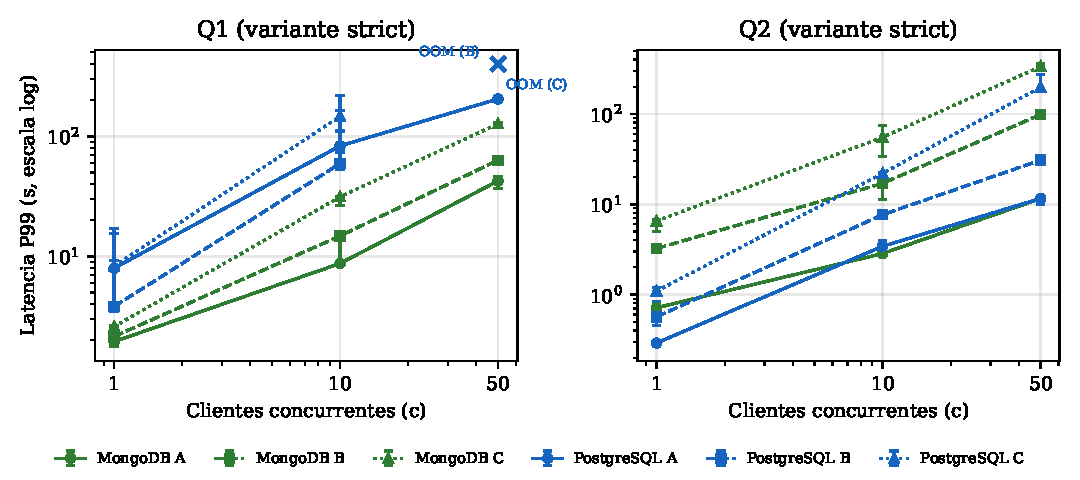
\includegraphics[width=\textwidth]{figuras/fig1_p99_concurrencia.pdf}
\caption{Latencia P99 frente a concurrencia (escalas logarítmicas). Mediana de 3 repeticiones; las barras indican el rango [mín, máx]. Las cruces señalan las celdas terminadas por OOM, que no tienen P99.}\label{fig:p99}
\end{figure}

En la figura~\ref{fig:p99} las pendientes son casi paralelas: con un motor saturado de CPU y clientes en lazo cerrado, la latencia crece proporcionalmente al número de clientes (ley de Little: $\text{latencia} \approx c/\text{QPS}$). Lo que distingue a los motores es el nivel y el punto de quiebre:
\begin{itemize}
  \item En Q1, la curva de PostgreSQL está entre 2 y 10 veces por encima de la de MongoDB en cada perfil y desaparece a $c=50$ en los perfiles B y C (OOM).
  \item En Q2, MongoDB en el perfil C es la curva más alta (334\,s de P99 con 50 clientes), por encima de PostgreSQL en el mismo perfil (197\,s).
\end{itemize}

\subsection{Throttling CFS frente a throughput}

\begin{figure}[H]
\centering
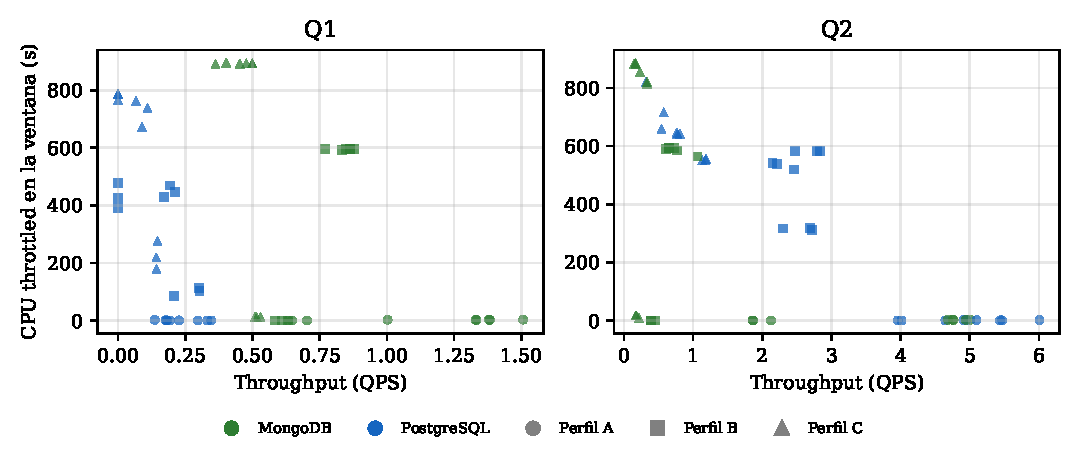
\includegraphics[width=\textwidth]{figuras/fig2_throttling_qps.pdf}
\caption{Tiempo de \emph{throttling} CFS en la ventana de 300\,s frente al throughput, por corrida (variante \texttt{strict}).}\label{fig:thr}
\end{figure}

La figura~\ref{fig:thr} muestra tres bandas horizontales: $\approx$0\,s (perfil A), $\approx$600\,s (perfil B) y $\approx$900\,s (perfil C). Esos valores son el techo teórico del \emph{throttling} cuando el contenedor tiene trabajo listo en las 4 CPUs de su \texttt{cpuset} durante toda la ventana: $(|\texttt{cpuset}| - \text{cuota}) \times 300\,\text{s}$, es decir $(4-2)\times300 = 600$\,s y $(4-1)\times300 = 900$\,s. MongoDB se acerca a ese techo con 10 o más clientes en B y C (585--597\,s y 821--894\,s); PostgreSQL lo alcanza incluso con un solo cliente en Q2 (316\,s en B y 552\,s en C), porque cada consulta lanza un líder y 2 \emph{workers} paralelos que compiten por la misma cuota.

\subsection{Evolución de la memoria}

\begin{figure}[H]
\centering
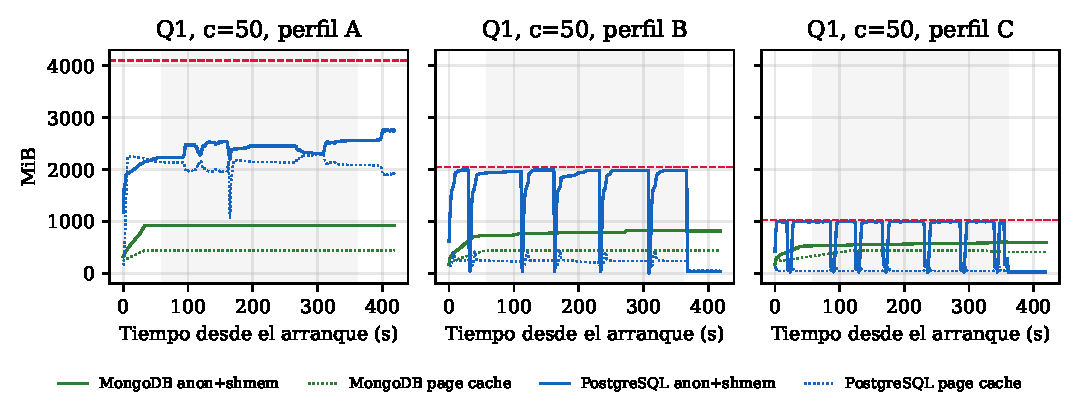
\includegraphics[width=\textwidth]{figuras/fig3_memoria_q1_c50.pdf}
\caption{Memoria del motor (\texttt{anon + shmem}, línea continua) y caché de páginas (\texttt{file}, punteada) en Q1 con 50 clientes, repetición 1. La línea roja es el límite del cgroup; la franja gris, la ventana de medición.}\label{fig:mem}
\end{figure}

La figura~\ref{fig:mem} es la evidencia directa de M2. MongoDB se mantiene plano por debajo de 1\,GB en los tres perfiles. PostgreSQL crece hasta $\approx$2.6\,GB en el perfil A (dentro de los 4\,GB) y en los perfiles B y C dibuja un patrón de diente de sierra: la memoria sube hasta el límite del cgroup, el kernel mata un \emph{backend}, el \texttt{postmaster} reinicia todos los procesos (recuperación) y el ciclo se repite durante toda la ventana.

\begin{figure}[H]
\centering
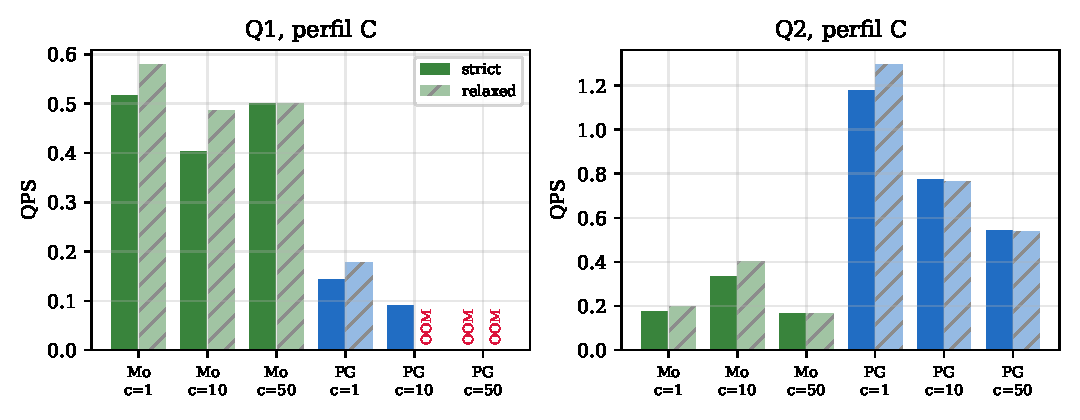
\includegraphics[width=\textwidth]{figuras/fig5_strict_relaxed_C.pdf}
\caption{Throughput con la variante \texttt{strict} (sólido) y \texttt{relaxed} (rayado) en el perfil C.}\label{fig:variantes}
\end{figure}

% =====================================================================
\section{Planes de ejecución}\label{sec:planes}

Los planes se obtuvieron con \texttt{explain("executionStats")} en MongoDB y \texttt{EXPLAIN (ANALYZE, BUFFERS, VERBOSE)} en PostgreSQL, fuera de la ventana de medición, en cada perfil y variante (24 planes en \texttt{results/explain/}). Los que se citan son del perfil C salvo que se indique otro.

\subsection{Q1 en PostgreSQL: estimación errónea, ordenamiento completo y volcado}

\begin{lstlisting}
GroupAggregate (rows=16504191 estimadas; actual rows=96)
  -> Incremental Sort   Pre-sorted Groups: 8  Sort Method: external merge  Peak Disk: 34336kB
     -> Nested Loop (actual rows=644159)
        -> Gather Merge   Workers Launched: 2   (rows=500000, width=1460)
           -> Sort  Sort Method: external merge  Disk: 221680kB   (líder)
                    Worker 0: external merge  Disk: 248680kB
                    Worker 1: external merge  Disk: 251064kB
              -> Parallel Seq Scan on orders (actual rows=166666 x 3)
        -> Function Scan on jsonb_array_elements item
              Filter: ((item.value->>'price')::numeric > 50)  Rows Removed by Filter: 2
Execution Time: 8041 ms   (perfil A: 5654 ms)
\end{lstlisting}

El planificador no tiene estadísticas sobre el contenido de \texttt{jsonb\_array\_elements} y estima \textbf{16.5 millones de grupos} frente a los 96 reales. Con esa estimación descarta \texttt{HashAggregate}, que no cabría en 4\,MB, y elige ordenar por país las 500\,000 filas \emph{completas} (\texttt{width=1460} bytes, el documento entero) antes de desanidar. Los 3 procesos vuelcan en conjunto $\approx$705\,MiB por ejecución, lo que coincide con los 30--81\,GiB de archivos temporales medidos por ventana (tabla~\ref{tab:m2}).

Con la variante \texttt{relaxed} (64\,MB), el \texttt{Incremental Sort} pasa a memoria (\texttt{quicksort}, pico 42\,MB), pero el \texttt{Sort} paralelo sigue en disco ($\approx$231--245\,MB por proceso, mayor que 64\,MB): el volcado se reduce, no desaparece.

\subsection{Q1 en MongoDB: agregación en flujo}

\begin{lstlisting}
$cursor  COLLSCAN  totalDocsExamined: 500000  (proyección temprana: customer.geo.country, items)
$unwind   nReturned: 1499046
$match    nReturned: 644159
$group    nReturned: 96    peakTrackedMemBytes: 64256   usedDisk: false   spills: 0
executionTimeMillis: 3486   (perfil A: 3229)
\end{lstlisting}

MongoDB proyecta sólo los dos campos necesarios, desanida en flujo y acumula directamente en una tabla hash de 96 entradas ($\approx$64\,KB). No necesita ordenar nada, por eso \texttt{allowDiskUse} es irrelevante para Q1 y el plan es idéntico en ambas variantes.

\subsection{Q2 en ambos motores: Top-N acotado y patrón de acceso}

\begin{lstlisting}
-- PostgreSQL
Limit -> Gather Merge (Workers Launched: 2)
  -> Sort  Sort Method: top-N heapsort  Memory: 276kB   (workers: 273kB, 272kB)
     -> Parallel Seq Scan on orders (rows estimadas 474; reales 60436 x 3)
Execution Time: 2561 ms   (perfil A: 2201 ms)
-- MongoDB
PROJECTION <- SORT (limitAmount: 1000, peakTrackedMemBytes: 1347009, usedDisk: false)
  <- FETCH (226680 docs) <- IXSCAN timestamp_1 (226680 claves)
executionTimeMillis: 9098   (perfil A: 5591)
\end{lstlisting}

Ambos motores reconocen el \texttt{LIMIT 1000} y mantienen sólo los 1\,000 mejores candidatos: 276\,KB en PostgreSQL y 1.35\,MB en MongoDB, muy por debajo de 4\,MB y de 100\,MB. Por eso Q2 nunca volcó y la variante de memoria no tuvo efecto: \textbf{Q2 funciona como control negativo de memoria}, no como estrés de buffer.

La diferencia de rendimiento la explica el patrón de acceso:
\begin{itemize}
  \item \textbf{MongoDB} usa el índice de \texttt{timestamp}, pero el filtro selecciona el 45\,\% de la colección; esto implica 226\,680 lecturas aleatorias de documentos (\texttt{FETCH}) para evaluar \texttt{payment.status}. Cuando la caché de WiredTiger se reduce a 0.5 y 0.25\,GB, esas lecturas dejan de estar en memoria y el tiempo pasa de 5.6\,s a 9.1\,s por ejecución.
  \item \textbf{PostgreSQL} ignora el índice y hace un recorrido secuencial paralelo, que con esa selectividad es más barato y menos sensible a la caché.
\end{itemize}

% =====================================================================
\section{Interpretación: límites de memoria, volcado a disco y throttling de cgroups}

\subsection{M1 --- ¿Cómo cambian P95/P99 al limitar CPU y memoria?}

\begin{table}[H]
\centering
\begin{threeparttable}
\caption{M1: P99 (s) por perfil y variación respecto del perfil A, a igual concurrencia (variante \texttt{strict}).}\label{tab:m1}
\scriptsize\setlength{\tabcolsep}{4pt}
\begin{tabular}{llrrrrrrrr}
\toprule
Q & Motor & $c$ & P99 A & P99 B & $\Delta$B & Thr. B (s) & P99 C & $\Delta$C & Thr. C (s) \\
\midrule
\tabinput{tablas/m1.tex}
\bottomrule
\end{tabular}
\begin{tablenotes}\scriptsize
\item $\Delta = (\text{P99}_X - \text{P99}_A)/\text{P99}_A$. En PostgreSQL Q1 a $c=1$ el P99 del perfil A está inflado por una repetición con cola larga (rango 3.46--9.32\,s) y por un tamaño de muestra menor a 100.
\end{tablenotes}
\end{threeparttable}
\end{table}

\begin{itemize}
  \item \textbf{La contención de CPU domina la cola.} Para MongoDB en Q1, el P99 a 10 clientes crece 70\,\% en B y 259\,\% en C, en paralelo con el \emph{throttling} (597 y 894\,s). Con un solo cliente la variación es pequeña (+10\,\% y +33\,\%) porque una consulta de MongoDB usa un solo hilo y no agota la cuota.
  \item \textbf{La contención de memoria cambia el tipo de fallo.} En PostgreSQL Q1, a $c=50$ el problema deja de ser la latencia y pasa a ser la estabilidad: OOM en B y en C.
  \item \textbf{En Q2 la degradación de MongoDB es la mayor de todo el experimento} (+753\,\% en B y +2\,802\,\% en C a $c=50$), porque al reducir el perfil se reduce también la caché de WiredTiger y el plan depende de lecturas aleatorias. PostgreSQL se degrada menos (+166\,\% y +1\,603\,\%).
\end{itemize}

\subsection{M2 --- ¿Qué motor gestiona mejor los buffers antes del volcado o del OOM?}

\begin{table}[H]
\centering
\begin{threeparttable}
\caption{M2: estado de las 3 repeticiones por celda y volumen de archivos temporales de PostgreSQL en la ventana (mediana).}\label{tab:m2}
\scriptsize\setlength{\tabcolsep}{4pt}
\begin{tabular}{lllllll}
\toprule
Q & Motor & Perfil & Variante & $c=1$ & $c=10$ & $c=50$ \\
\midrule
\tabinput{tablas/m2.tex}
\bottomrule
\end{tabular}
\begin{tablenotes}\scriptsize
\item Los GiB son el incremento de \texttt{pg\_stat\_database.temp\_bytes} en los 300\,s de medición. En las celdas \texttt{oom} ese contador no es utilizable: la recuperación tras el OOM lo reinicia a cero.
\end{tablenotes}
\end{threeparttable}
\end{table}

\textbf{MongoDB gestionó mejor los buffers en esta carga}: 0 volcados y 0 OOM en 90 corridas, con una huella de estado de agregación de 64\,KB (Q1) y 1.35\,MB (Q2). PostgreSQL volcó en el 100\,\% de las corridas de Q1 que terminaron y alcanzó el OOM en 12 corridas. Las causas son dos:
\begin{enumerate}
  \item \textbf{Una estimación de cardinalidad errónea} sobre la salida de \texttt{jsonb\_array\_elements} lleva a un plan que ordena el documento completo en lugar de agregar en hash. Es una limitación de JSONB (sin estadísticas sobre el contenido), no del almacenamiento en sí.
  \item \textbf{\texttt{work\_mem} se aplica por operación y por proceso.} Con 50 sesiones, cada una con líder y 2 \emph{workers} y varios nodos de ordenamiento, la memoria privada se multiplica hasta superar el límite del cgroup.
\end{enumerate}

\paragraph{Hipótesis dual sobre \texttt{relaxed}: confirmada.} En el perfil C (tabla~\ref{tab:anexo} y figura~\ref{fig:variantes}), \texttt{work\_mem = 64MB} aumentó el throughput de PostgreSQL con 1 cliente de 0.143 a 0.177 QPS (+24\,\%; menos pases de mezcla). Pero con 10 clientes convirtió el \texttt{spill} en \texttt{oom} en las 3 repeticiones (60 eventos \texttt{oom\_kill}): a mayor límite por operación, más memoria privada concurrente y menos margen bajo un techo fijo sin swap. Con 50 clientes ambas variantes terminan en OOM. En MongoDB y en Q2 la variante no cambió el plan.

\subsection{M3 --- Huella de CPU y memoria por cada 1\,000 documentos}

\begin{table}[H]
\centering
\begin{threeparttable}
\caption{M3 (variante \texttt{strict}, mediana de 3 repeticiones). Mo = MongoDB, PG = PostgreSQL.}\label{tab:m3}
\scriptsize\setlength{\tabcolsep}{4pt}
\begin{tabular}{lllrrrrrr}
\toprule
 & & & \multicolumn{2}{c}{CPU$_{1k}$ (ms CPU)} & \multicolumn{2}{c}{Mem$_{\text{peak}}$ (MB)} & \multicolumn{2}{c}{Mem$_{1k}$ (MB$\cdot$s)} \\
\cmidrule(lr){4-5}\cmidrule(lr){6-7}\cmidrule(lr){8-9}
Q & $c$ & Perfil & Mo & PG & Mo & PG & Mo & PG \\
\midrule
\tabinput{tablas/m3.tex}
\bottomrule
\end{tabular}
\begin{tablenotes}\scriptsize
\item CPU$_{1k}$ y Mem$_{1k}$ se normalizan por consultas completadas $\times$ 500\,000 documentos; no se definen cuando no se completó ninguna consulta (celdas \texttt{oom}). Mem$_{\text{peak}}$ es un nivel y no se normaliza: incluye \texttt{shared\_buffers} (PostgreSQL) y la caché de WiredTiger (MongoDB).
\end{tablenotes}
\end{threeparttable}
\end{table}

\begin{figure}[H]
\centering
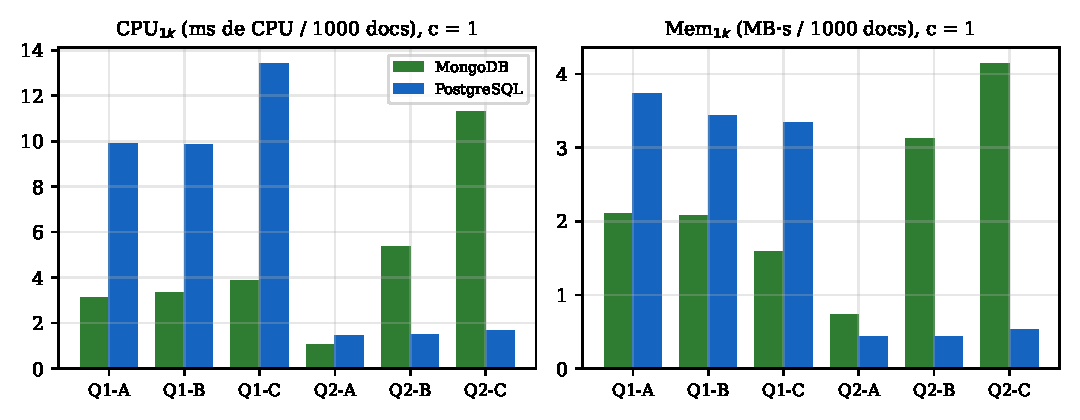
\includegraphics[width=\textwidth]{figuras/fig4_m3_c1.pdf}
\caption{M3 con un cliente: CPU y memoria integrada por cada 1\,000 documentos.}\label{fig:m3}
\end{figure}

\begin{itemize}
  \item \textbf{Q1:} PostgreSQL consume entre 2.9 y 3.5 veces más CPU por cada 1\,000 documentos que MongoDB a $c=1$ (9.9--13.4 frente a 3.1--3.9\,ms). La diferencia crece con la concurrencia (17.8--22.9\,ms a $c\ge10$) porque los procesos compiten por E/S de volcado. Es decir, el costo de desanidar y ordenar documentos JSONB completos es mayor que el de recorrer BSON con proyección temprana.
  \item \textbf{Q2:} PostgreSQL es más eficiente y estable (1.4--1.7\,ms en todos los perfiles a $c=1$). MongoDB es comparable en A (1.1\,ms) pero sube a 5.4 y 11.3\,ms en B y C: las lecturas aleatorias que fallan en caché se pagan en CPU (descompresión de páginas) y en tiempo.
  \item \textbf{Memoria:} el pico de PostgreSQL incluye \texttt{shared\_buffers} y crece con la concurrencia (hasta 2.6\,GB en Q1, A, $c=50$); el de MongoDB está acotado por la caché de WiredTiger (387--922\,MB). La memoria integrada por documento (Mem$_{1k}$) favorece a MongoDB en Q1 y a PostgreSQL en Q2, igual que la CPU.
\end{itemize}

\subsection{Throttling de cgroups y paralelismo intra-consulta}\label{sec:throttling}

El \emph{throttling} reportado puede superar los 300\,s porque el kernel lo acumula por CPU del \texttt{cpuset}; su techo es $(4-\text{cuota})\times300$\,s. Dos lecturas se desprenden de los datos:
\begin{itemize}
  \item Con una cuota de 1 o 2 CPUs y 4 CPUs disponibles en el \texttt{cpuset}, el paralelismo intra-consulta de PostgreSQL (\texttt{max\_parallel\_workers\_per\_gather = 2}) no aporta capacidad: los 3 procesos agotan la cuota antes y pasan el resto del periodo bloqueados. En Q2 con 1 cliente, PostgreSQL acumula 552\,s de \emph{throttling} en C, mientras MongoDB, de un solo hilo por consulta, acumula 17\,s.
  \item Con suficientes clientes, ambos motores llegan al techo: la cuota CFS, no el motor, es el cuello de botella. A partir de ese punto, más concurrencia sólo alarga la cola (figura~\ref{fig:p99}).
\end{itemize}

\subsection{Respuestas a las preguntas del revisor}

\begin{enumerate}[label=\textbf{\arabic*.}]
  \item \textbf{¿El baseline es comparable (mismo dataset, mismas consultas)?} Sí. Ambos motores cargaron el mismo NDJSON (SHA-256 verificado) y devolvieron los mismos conteos y la misma suma de \texttt{final\_total}; las consultas son las del playbook sin modificaciones; las imágenes están fijadas por digest; el perfil A usa la misma configuración de caché por fabricante que B y C.
  \item \textbf{¿Las latencias son P50/P95/P99 o sólo promedios?} Son percentiles calculados sobre cada consulta individual de la ventana. Se reporta $n$ por celda y se marcan con $\dagger$ las 19 de 60 celdas con alguna repetición de menos de 100 consultas.
  \item \textbf{¿Hubo throttling CFS? ¿Cuántos segundos?} Sí, en los perfiles B y C: hasta 597\,s y 894\,s por ventana, coherentes con el techo teórico de 600 y 900\,s (tablas~\ref{tab:resq1}, \ref{tab:resq2} y~\ref{tab:m1}; figura~\ref{fig:thr}). En el perfil A fue prácticamente nulo ($\leq$3\,s).
  \item \textbf{¿Spill a disco u OOM? ¿En qué perfil y concurrencia?} Volcado: PostgreSQL Q1 en todas las celdas que terminaron (A, B y C; $c$ = 1 y 10, y $c=50$ en A). OOM: PostgreSQL Q1 con $c=50$ en B y C (\texttt{strict}) y con $c$ = 10 y 50 en C (\texttt{relaxed}). MongoDB y Q2: ninguno (tabla~\ref{tab:m2}).
  \item \textbf{¿Cuántas repeticiones y cómo se resume?} Tres por celda; se reporta la mediana y el rango [mín, máx]. No se promedian percentiles.
  \item \textbf{¿El plan de ejecución respalda el cuello de botella?} Sí: \texttt{external merge} con $\approx$705\,MiB por ejecución y una estimación de 16.5\,M de grupos en PostgreSQL Q1; agregación hash de 64\,KB en MongoDB Q1; \texttt{top-N heapsort} de 276\,KB frente a IXSCAN + 226\,680 \texttt{FETCH} en Q2 (sección~\ref{sec:planes}).
\end{enumerate}

\subsection{Amenazas a la validez y limitaciones}\label{sec:amenazas}

\begin{enumerate}[label=\textbf{\arabic*.}]
  \item \textbf{Entorno virtualizado en lugar de Linux nativo.} Los contenedores corrieron sobre el kernel Linux de la VM de WSL2 (Docker Desktop), no sobre un anfitrión Linux. Los mecanismos medidos (CFS, \texttt{memory.max}, OOM-killer, \texttt{cpu.stat}, \texttt{memory.stat}) son los del kernel Linux, pero:
  \begin{itemize}
    \item las CPUs del \texttt{cpuset} son CPUs virtuales que Hyper-V reparte entre núcleos P y E del procesador híbrido, por lo que el rendimiento por CPU no es constante;
    \item la E/S de los volcados de PostgreSQL atraviesa el disco virtual de la VM, lo que probablemente penaliza más a PostgreSQL que un disco nativo;
    \item el control de ruido (CPUs ociosas) sólo observa la VM, no la carga de Windows.
  \end{itemize}
  Ambos motores se midieron en el mismo entorno, con orden aleatorio y los mismos filtros de calidad, por lo que las \emph{comparaciones} entre motores y perfiles son válidas; los valores absolutos no deben extrapolarse a un servidor Linux.
  \item \textbf{Runner fuera de la VM.} Los clientes corrieron en Windows y llegaron a los motores por el reenvío de puertos de Docker Desktop. Esto añade latencia de red local del orden de milisegundos (despreciable frente a latencias de segundos) y compite por los mismos núcleos físicos que la VM.
  \item \textbf{Degradación periódica de Docker Desktop.} Durante la campaña, Docker Desktop/WSL2 se degradó tras $\approx$1--1.5\,h de uso continuo (lecturas lentas de cgroups, comandos de Docker lentos). Esto produjo 31 intentos descartados y 3 detenciones, y se mitigó con 18 pausas para reiniciar Docker Desktop y WSL entre corridas (anexo~\ref{anx:incidencias}). Ninguna corrida degradada llegó al CSV: todas fallaron el control de muestras y se repitieron.
  \item \textbf{Censura por la ventana de 300\,s.} En las celdas con consultas de decenas o cientos de segundos, las consultas que no terminan dentro de la ventana no se observan, por lo que el P99 está truncado (19 celdas con $n<100$, marcadas con $\dagger$). Las celdas \texttt{oom} no tienen latencias.
  \item \textbf{Variabilidad entre corridas.} En celdas donde la variante no cambia el plan, las diferencias llegaron a $\pm$20\,\% (tabla~\ref{tab:anexo}); diferencias menores a ese margen no deben interpretarse como efectos.
  \item \textbf{Cambios operativos durante la campaña.} El plan se amplió de 144 a 180 corridas (Q2 \texttt{relaxed} en A y B) y el tope de incidencias del orquestador se elevó de 4 a 12. Ninguno modificó consultas, perfiles, telemetría ni código de medición: un manifiesto SHA-256 de 21 archivos protegidos se verificó intacto antes de cada reanudación, y las 144 corridas originales conservaron su orden.
  \item \textbf{Índice de \texttt{timestamp} en PostgreSQL} habilitado modificando \texttt{pg\_catalog}; no es reproducible en servicios administrados (aunque el planificador no lo usó en Q2).
\end{enumerate}

% =====================================================================
\section{Recomendaciones técnicas para despliegues documentales en la nube}\label{sec:recomendaciones}

\subsection{Respaldadas directamente por los resultados}

\begin{enumerate}
  \item \textbf{Elegir el motor según el patrón de consulta, no por el modelo de datos.} Para agregaciones que desanidan arreglos y agrupan (tipo Q1), MongoDB obtuvo entre 1.9 y 7.4 veces más throughput, sin volcado y sin OOM. Para filtros amplios con Top-K (tipo Q2), PostgreSQL fue más rápido y menos sensible a la reducción de memoria.
  \item \textbf{Dimensionar \texttt{work\_mem} contra el límite del contenedor, no contra una consulta aislada.} Con \texttt{memory.swap.max = 0}, una cota práctica es
  \[\texttt{work\_mem} \lesssim \frac{\text{límite} - \texttt{shared\_buffers}}{\text{sesiones} \times (1 + \text{workers}) \times \text{nodos de ordenamiento}}.\] Subirlo de 4 a 64\,MB convirtió volcados en OOM con 10 sesiones en 1\,GB.
  \item \textbf{Limitar el paralelismo intra-consulta cuando la cuota CFS es pequeña.} Con 1--2 vCPU, \texttt{max\_parallel\_workers\_per\_gather} en 0 o 1 evita que 3 procesos por consulta se estrangulen mutuamente (552\,s de \emph{throttling} con un solo cliente en Q2, perfil C).
  \item \textbf{Limitar la concurrencia en PostgreSQL con un pool} (por ejemplo, PgBouncer) en contenedores pequeños: el OOM apareció con 50 sesiones en 2\,GB, no con 10.
  \item \textbf{En MongoDB, dimensionar la caché de WiredTiger según el conjunto de trabajo de las consultas con \texttt{FETCH} aleatorio.} Reducirla de 1.5 a 0.25\,GB multiplicó por 9 la latencia de Q2 a 1 cliente; fijar siempre \texttt{-{}-wiredTigerCacheSizeGB} según el límite del contenedor.
  \item \textbf{Medir con percentiles y \emph{throttling}, no sólo con CPU promedio.} El \emph{throttling} explicó la cola de latencia aun cuando el uso de CPU parecía igual a la cuota.
\end{enumerate}

\subsection{Buenas prácticas generales (no medidas directamente)}

\begin{itemize}
  \item En PostgreSQL con JSONB, materializar los campos que se agrupan o filtran con frecuencia (columnas generadas \texttt{STORED} o tablas normalizadas) para que el planificador tenga estadísticas y elija \texttt{HashAggregate}.
  \item En servicios administrados (RDS, Cloud SQL, Azure) no se puede modificar \texttt{pg\_catalog}: para indexar fechas en JSONB, usar una función \texttt{IMMUTABLE} propia o extraer el valor a una columna \texttt{timestamptz}.
  \item Usar \texttt{allowDiskUse: true} en MongoDB sólo con concurrencia acotada en etapas \texttt{\$group}/\texttt{\$sort} de alta cardinalidad.
  \item Validar en el entorno de producción (Linux nativo o el servicio administrado) los valores absolutos de este estudio, obtenidos en una VM de WSL2.
\end{itemize}

% =====================================================================
\appendix

\section{Registro de incidencias de la campaña}\label{anx:incidencias}

La campaña empezó el 31 de octubre de 2026 a las 02:02 y terminó el 1 de noviembre a las 14:44 (36.7\,h de reloj). La tabla~\ref{tab:incidencias} resume el journal del orquestador (\texttt{state/journal.jsonl}).

\begin{table}[H]
\centering\small
\caption{Eventos operativos registrados en el journal.}\label{tab:incidencias}
\begin{tabular}{lr}
\toprule
Corridas iniciadas / registradas & 211 / 180 \\
Intentos descartados y repetidos & 31 \\
\quad por \texttt{telemetry\_gap} (menos de 240 muestras) & 24 \\
\quad por \texttt{runner\_exception} (clientes sin sincronizar en 60\,s) & 3 \\
\quad por \texttt{compose\_failed} / \texttt{engine\_start\_failed} / \texttt{drop\_caches\_failed} & 2 / 1 / 1 \\
Incidencias abiertas por el orquestador & 9 \\
Detenciones (\texttt{halted}) & 3 \\
Pausas para reinicio preventivo de Docker Desktop y WSL & 18 \\
\bottomrule
\end{tabular}
\end{table}

Los intentos descartados no se escribieron en el CSV. Tras cada detención o reinicio se verificó con \texttt{doctor} que el manifiesto SHA-256 de los archivos protegidos y el dataset no hubieran cambiado antes de reanudar.

\section{Reproducibilidad}

\begin{lstlisting}[language=bash]
python synthetic_data_generator.py --n 500000 --seed 42 --out-dir data   # SHA-256 9cd202a6...
docker compose pull
./run_benchmarks.sh doctor          # verificaciones previas
./run_benchmarks.sh load-data       # carga y verificación de paridad
./run_benchmarks.sh start           # 180 corridas, plan con semilla 20261030
./run_benchmarks.sh summarize       # medianas y rangos por celda
\end{lstlisting}

Archivos de evidencia:
\begin{itemize}
  \item \texttt{results/mediciones.csv} (108 filas) y \texttt{results/anexo\_variantes.csv} (72 filas);
  \item \texttt{results/raw/<run\_id>/} con \texttt{meta.json}, \texttt{series.csv} (1\,Hz) y \texttt{latencies.jsonl} (cada consulta);
  \item \texttt{results/explain/} (24 planes);
  \item \texttt{state/journal.jsonl} y \texttt{state/plan.json}.
\end{itemize}

\section{Esquema del CSV de mediciones}

\begin{lstlisting}
timestamp_epoch,engine,profile,query_id,concurrency,run_number,throughput_qps,
latency_p50_ms,latency_p95_ms,latency_p99_ms,cpu_throttled_seconds,max_rss_mb,disk_spill,status
\end{lstlisting}

Esquema idéntico al de la sección~8.2 del playbook. \texttt{query\_id} toma los valores \texttt{Q1}, \texttt{Q2}, \texttt{Q1\_relaxed} y \texttt{Q2\_relaxed}; \texttt{status} toma \texttt{ok}, \texttt{spill}, \texttt{oom} o \texttt{error}.

\end{document}
